\section{Datathons}


3. Datathons
- describe what a datathon is
3.1 Benefits
3.2 DFG Case Study
3.3 CODE Case Study
4. Discussion (Lessons Learned)
- community engagement
- participants: recruitment, group dynamics
- data: structuring and cleaning, open data, storing
- tools: analysis, visualization
- logistics: room setup, break out rooms, food
- things to avoid
5. Conclusions


 ? Intro
 ? Related Work
 ? Datathons in general
  ? benefits
  ? Two hackathon case studies
   � Code
    ? Recruitment - population of attendees
    ? Preparing data
    ? Setup
    ? Group dynamics
   � DfG
 ? Lessons Learned
  ? How to do, tips
  ? Things to avoid

%----------------------------------------------------
% PREPARATION and PLANNING
%----------------------------------------------------
\section{Preparation and Planning}

%----------------------------------------------------
% RECRUITMENT
%----------------------------------------------------
\subsection{Recruitment}

%----------------------------------------------------
% VENUE
%----------------------------------------------------
\subsection{Venue}

%\begin{figure}[!t] % this puts images exactly where you want them
%\begin{center}
%\subfigure[Expectations of the course from students.]{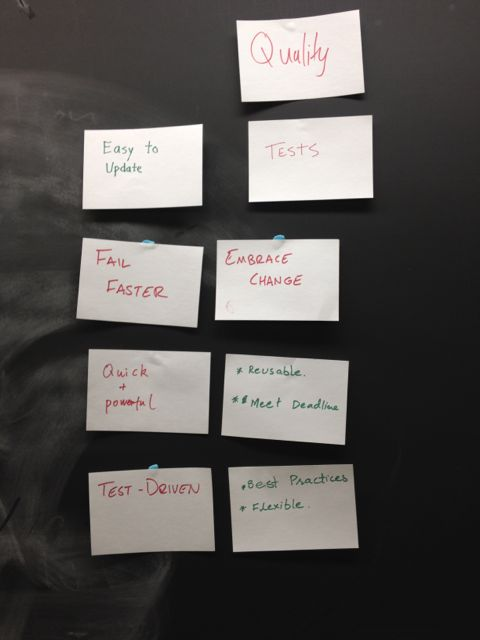
\includegraphics[keepaspectratio,width=4.1cm]{images/expectations.png}\label{fig:expectations}}
%\subfigure[Marshmallow Challenge: students working in teams.]{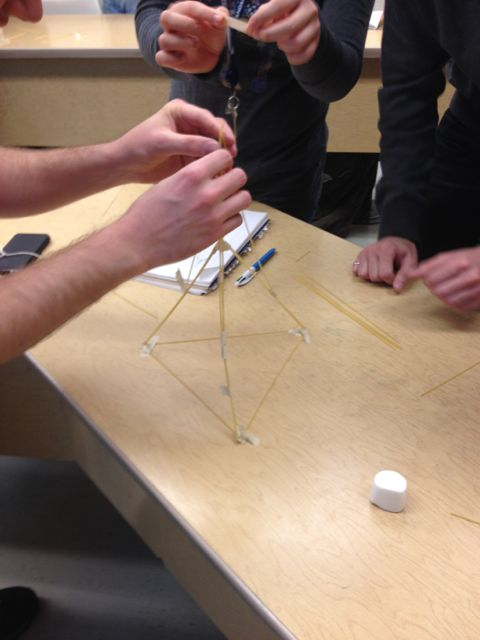
\includegraphics[keepaspectratio,width=4.1cm]{images/marshmallow.png}\label{fig:marshmallow}}
%\caption{Course Lectures - interactive exercises.}
%\label{fig:lectures}
%\end{center}
%\end{figure}
%

%----------------------------------------------------
% DATA PREPARATION
%----------------------------------------------------
\subsection{Data Preparation}

%----------------------------------------------------
% LOGISTICSs
%----------------------------------------------------
\subsection{Logistics}

%----------------------------------------------------
% HOSTING
%----------------------------------------------------
\section{Hosting the Event}
